%%
%% ****** ljmsamp.tex 13.06.2018 ******
%%
\documentclass[
11pt,%
tightenlines,%
twoside,%
onecolumn,%
nofloats,%
nobibnotes,%
nofootinbib,%
superscriptaddress,%
noshowpacs,%
centertags]%
{revtex4}
\usepackage{ljm}
% \usepackage{cmap}					% поиск в PDF
% \usepackage{mathtext} 				% русские буквы в формулах
% \usepackage[T2A]{fontenc}			% кодировка
%\usepackage[utf8x]{inputenc}			% кодировка исходного текста
%\usepackage[russian]{babel}	% локализация и переносы

\begin{document}

%\titlerunning{Численное решение волнового уравнения} % for running heads
%\authorrunning{\firstname{Д.~Ю.}~\surname{Бобрышев}} % for running heads
%\authorrunning{First-Author, Second-Author} % for running heads

\title{Численное решение волнового уравнения}
% Splitting into lines is performed by the command \\
% The title is written in accordance with the rules of capitalization.

\author{\firstname{Д.~Ю.}~\surname{Бобрышев}}
\email[E-mail: ]{bobryshev.diu@phystech.edu}
%\affiliation{Place of work and/or the address of the first and second authors}
\affiliation{Московский физико-технический институт, Институтский пер., 9, Долгопрудный, Московская обл., 141701}

\author{\firstname{С.~М.~М.}~\surname{Аль-Хадж Аюб}}
\email[E-mail: ]{al-khadzh.aiub.sm@phystech.edu}
%\affiliation{Place of work and/or the address of the first and second authors}
%\affiliation{Place of work and/or the address of second authors}
%\noaffiliation % If the author does not specify a place of work.

%\firstcollaboration{(Submitted by Я)} % Add if you know submitter.
%\lastcollaboration{ }

\received{22 Мая, 2024} % The date of receipt to the editor, i.e. December 06, 2017


\begin{abstract} % You shouldn't use formulas and citations in the abstract.
Основной целью данной работы является наблюдение различных эффектов, возникающих при решении волнового
уравнения. Численное решение выполнено при помощи метода конечных элементов, написано на языке C++ 
с использованием библиотеки FEniCS. 


\end{abstract}

%\subclass{12345, 54321} % Enter 2010 Mathematics Subject Classification.

\keywords{Волновое уравнение, FEniCS} % Include keywords separeted by comma.

\maketitle

% Text of article starts here.

\section{Введение}
Волновое уравнение (1) является одним из основных уравнений математической физики. При помощи
волнового уравнения описываются различные колебательные процессы, например, 
распространение звуковой волны в среде, распространение электромагнитных волн. В данной работе
мы будем использовать теорминологию, используемую в электродинамике, а полученное решение 
следует интерпретировать как распространение электромагнитной волны. \newline
\begin{equation}
    \Delta u = \frac{1}{v^2}\frac{\partial^2u}{\partial t^2}
\end{equation}
При решении волнового уравнения возникает ряд интересных эффектов. Например, выполняется принцип
Гюйгенса-Френеля: каждая точка волнового фронта является источником вторичных
когерентных сферических волн. При некоторых условиях, как следствие этого приниципа, 
имеет место дифракция: явление огибания предметов световой волной. Так, например, если осветить
узкую щель плоской монохроматической волной, на достаточно удалённом экране можно наблюдать
последовательность светлых полос. Наблюдение дифракции является одной из основных целей
работы.\newline
Из принципа Гюйгенса-Френеля следует закон преломления волны при прохождении границы двух сред
с различными показателями преломления. Преломлённая волна имеет иную скорость распространения, поэтому
у преломлённой волны угол между направлением распространения и нормалью к поверхности оказывается
иным, чем угол между нормалью и направлением распространения падающей волны. Данное явление
можно использовать, например, для фокусировки волны в точку. Для этого используются
линзы. Исследование свойств линз также является важной частью работы. \newline
Для решения волнового уравнения мы использовали метод конечных элементов. Основной идеей данного
метода является разбиение пространства, на котором необходимо получить решение, на некоторое
конечное количество элементов: точек со связывающих их отрезками. Для каждой пары отрезков, имеющих
общую точку, можно ввести линейную функцию $v_k$, и число $u_k$, а саму функцию аппроксимировать как
сумму базисных функций $v_k$, умноженных на коэффициент $u_k$. Таким образом, дифференциальное уравнение
с некоторыми граничными условиями можно приближённо представить в виде системы линейных уравнений,
которую можно решить относительно $u_k$, и, таким образом, получить приближённо функцию u. Метод 
конечных элементов реализован в библиотеке FEniCS, которую мы использовали для получения численного
решения волнового уравнения.


\section{Теоретическая часть}
\subsection{Дифракционная решётка}
В данной работе используется пропускающая дифракционная решётка, состоящая из чередующихся пропускающих
полосок, называемых щелями, шириной a и не пропускающих полосок шириной b. Величина d = a + b называется
периодом дифракционной решётки. Распределение интенсивности света, прошедшего через дифракционную
решётку, на удалённом экране:
\begin{equation}
    I = I_0 \frac{\sin^2(n\nu)}{\sin^2(\nu)}\frac{\sin^2(u)}{u^2},
\end{equation}  
где 
\begin{equation}
    u = \frac{\pi}{\lambda} a \sin(\varphi),
\end{equation}
\begin{equation}
    \nu = \frac{\pi}{\lambda} d \sin(\varphi).
\end{equation}
Здесь $\varphi$ - направление  от дифракционной решётки на рассматриваемую точку экрана, $\lambda$ - 
длина волны падающего света. 
На экране получается следующее распределение интенсивности:
\begin{figure}[h]
    \centering
    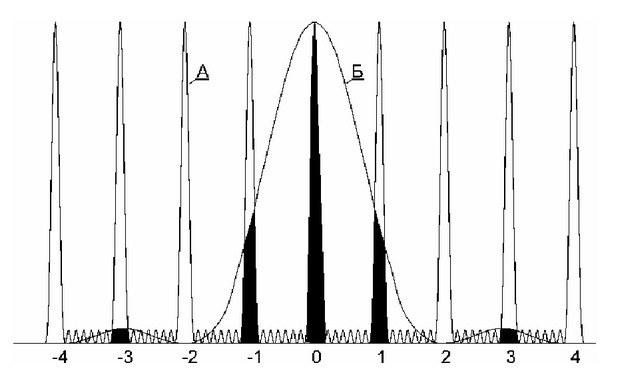
\includegraphics[width=10cm]{intensity.jpg}
    \caption{Распределение интенсивности на удалённом экране}
    \label{fig:1}
\end{figure}
\newline
Угловое положение главных максимумов:
\begin{equation}
    d\sin(\varphi) = m\lambda.
\end{equation}

\subsection{Аберрации света}
При рассмотрении хода лучей в геометрической оптике обычно считают выполненными следующие условия:
\begin{enumerate}
    \item свет постуапет в систему в виде параксиальных пучков
    \item пучки составляют небольшие углы с главной осью системы
    \item показатель преломления постоянен для всех лучей, т.е. среда не имеет дисперсии или свет достаточно монохроматичен
\end{enumerate}
Аберрациями называют отклонения луча от направления, по которому луч должен был бы идти в идеальной 
системе. Мы будем изучать сферическую аберрацию, которая возникает при невыполнении условия (1).
Сферическая аберрация обусловлена тем, что пучки света, падающие на разных расстояниях от линзы,
соберутся в различных точках на главной оптической оси. Так, параксиальный пучок соберётся в точке 
L', а пучок, прошедший через край линзы соберётся в точке L'''(см. рис. 2).
\begin{figure}[h]
    \centering
    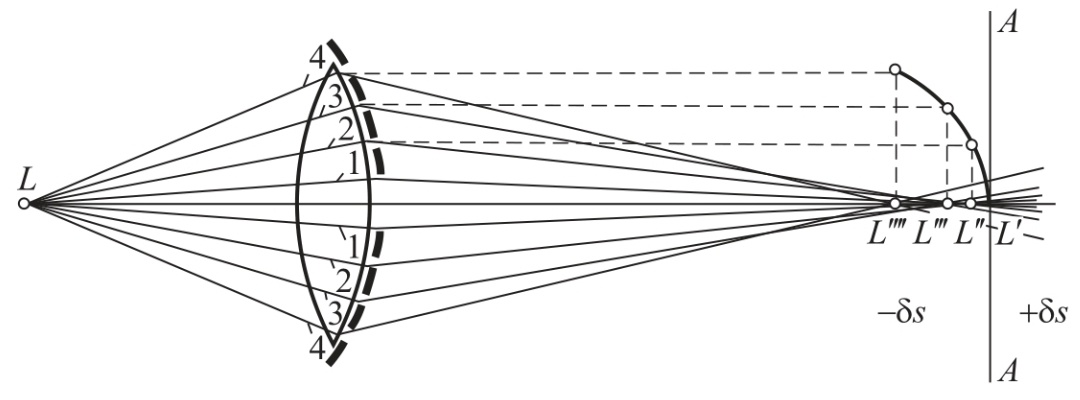
\includegraphics[width=10cm]{Spherical_aberration.jpg}
    \caption{Сферическая Аберрациями}
    \label{fig:1}
\end{figure}
Мерой продольной сферической аберрации можно считать расстояние L'L'''. Проведём через точку L' 
плоскость, перпендикулярную главной оптической оси. Луч, прощедший через край линзы, пересечёт эту
плоскость в некоторой точке A. Расстояние L'A называется поперечной сферической аберрацией. Второй
целью работы является измерение продольной и поперечной сферических аберраций. 


\section{Эксперимент}
\subsection{Вычисления}
Для решения волнового уравнения (1) мы выбрали следующий алгоритм. Производную по времени можно
представить так:
\begin{equation}
    \frac{\partial u}{\partial t} = \frac{u(t) - u(t-dt)}{dt}.
\end{equation}
Вторую производную, соответственно, следующим образом:
\begin{equation}
    \frac{\partial^2u}{\partial t^2} = \frac{u(t) + u(t-2dt) - 2u(t-dt)}{dt^2}.
\end{equation}
Таким образом, для вычисления поля $u$ в момент времени $t$ необходимо знать поле в два предыдущих
момента времени. Тогда можно задать необходимое поле в первые два момента времени, например, нулевое
поле в каждой точке. Затем добавить граничное условие и вычислить поле по формуле $dt^2 \Delta u = 
\frac{u}{v^2}$. После этого, сохранив результат вычисления, решить уравнение (1) с помощью формулы
(7). Таким итерационным методом можно получить поле $u(t)$ с заданными граничными условиями
в любой момент времени $t$. Мы будем использовать прямоугольную форму сетки, на которой будем 
вычислять поле. \newline
Отдельно нужно уделить внимание граничным условиям. Как известно, если у струны закрепить концы, 
волна, возбуждённая в струне, будет отражаться от концов. В данном случае также можно наблюдать
отражение волн от границ, причём стандартные граничные условия при решении с помощью библиотеки
FEniCS подразумевают отражение от границ с сохранением знака поля. При задании нулевого граничного
условия волна отразится с изменением знака. При этом отражённая волна может серьёзно повлиять
на результаты эксперимента. Поэтому подавление отражённой волны является одной из главных проблем
эксперимента. \newline
Погасить волну можно несколькими способами. Первый способ - добавление пространственного трения, 
т.е. добавление в уравнение (1) свёртки градиента функции. Оказалось, что так волна действительно
затухает, если добавить такое слагаемое во всём пространстве. Однако при попытке задать такое трение
в какой-то конкретной области, волна полностью отражается от этой области. Таким образом, погасить
волну таким способом не получится, потому что волна никак не окажется в области с трением, если она 
ранее была в области без трения. \newline
Второй способ - добавление вязкого трения, т.е. добавление в уравнение (1) члена вида 
$\eta \cdot \frac{\partial u}{\partial t}$. Если добавить такое слагаемое во всём пространстве, волна
затухает точно так же, как в случае с пространственным трением; однако при выделении отдельной области
с таким слагаемым волна не полностью отразится от этой области. При увеличении коэффициента $\eta$ 
доля отражённой волны будет возрастать, но затухание происходит быстрее. Далее мы увидим, что 
подобный способ погашения волны также не очень эффективен. \newline
Третий способ избавления от отражённой волны - введение достаточно большой сетки. Пространство для 
расчёта можно продлить в месте, где происходит отражение. Для того, чтобы время 
расчёта осталось примерно таким же, нужно сделать такую сетку разреженной. Это можно сделать потому, 
что информация о прошедшей волне нам не нужна, поэтому точность расчёта можно сделать очень малой. 
Этот способ является наиболее эффективным. \newline
При расчёте также необходимо учитывать численную вязкость: если расчёт происходит недостаточно точно,
проходящая волна начинает затухать. Для подавления этого эффекта нужно ставить достаточно малый шаг
по времени и достаточно большую частоту сетки.

\subsection{Дифракционная решётка}
Дифракционную решётку можно задать двумя способами. Первый способ - возбудить плоскую волну, падающую
на экран, на котором сделаны отверстия. Экран можно прописать в граничных условиях расчёта, т.е. 
сделать некоторую небольшую область, в которой поле всегда зануляется. Но, как указано в предыдущем 
пункте, волна начнёт отражаться от экрана. Отражённая волна может снова отразиться от границы и второй
раз попасть на экран, что может немного испортить картину. Можно сделать экран как область с трением. 
В таком случае часть волны поглотится, а часть отразится. Однако полностью поглотиться волна не сможет.
Если сделать трение слишком большим, отражённая волна, как и в предыдущем случае, может повлиять на 
расчёт. Если сделать трение достаточно малым, чтобы не замечать отражённую волну, прошедшая волна 
не затухнет до конца и также повлияет на результат эксперимента. Поэтому более предпочтительным 
является второй способ, менее естественный, но более эффективный. \newline
\begin{figure}[h]
    \centering
    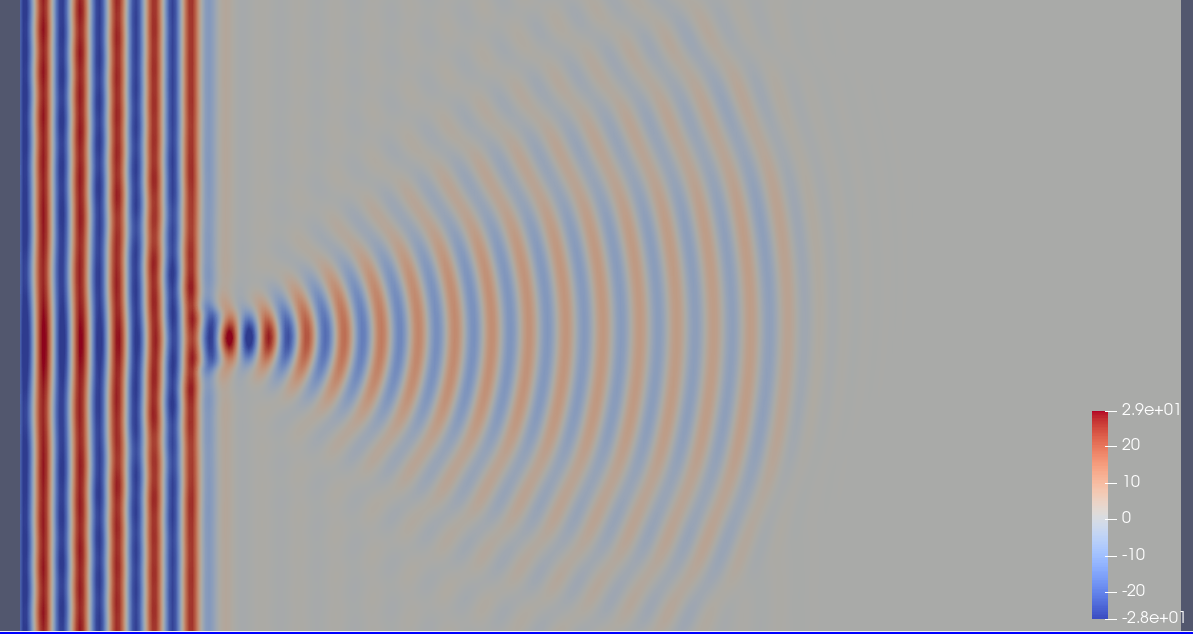
\includegraphics[width=13cm]{Field_with_one_gap.png}
    \caption{Распределение напряжённости электрического поля за экраном с одной щелью}
    \label{fig:1}
\end{figure}

Второй способ - задание граничных условий, соответствующих состоянию волны сразу за дифракционной 
решёткой. Такой способ имеет ряд преимуществ: нет влияния отражённой и прошедшей сквозь экран волн, 
не нужно просчитывать область между экраном и левой границей. Именно этот способ мы использовали для 
последнего расчёта. Кроме того, мы использовали большую сетку, которая становится разреженной ближе
к краю.
\newpage
\begin{figure}[h]
    \centering
    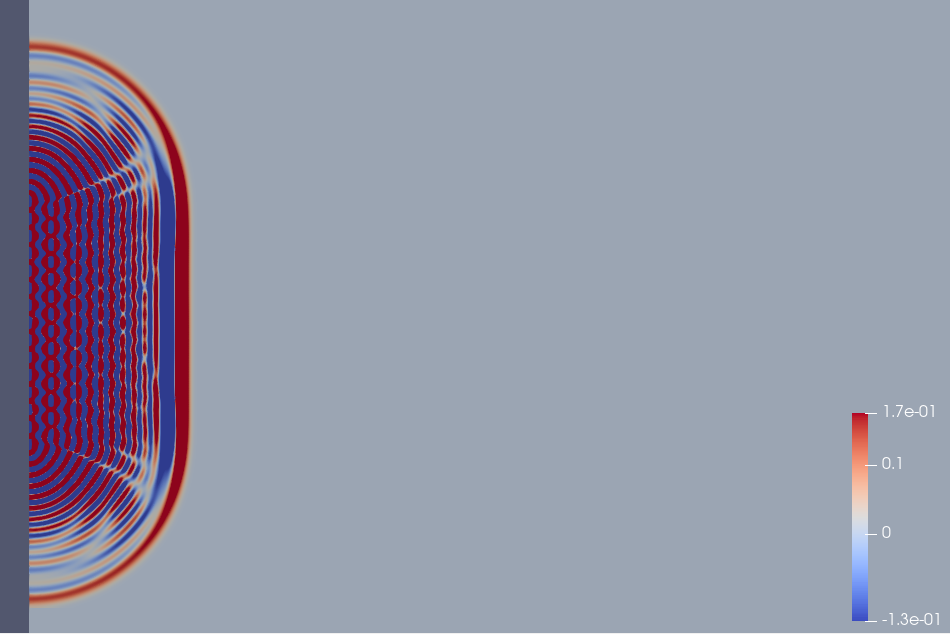
\includegraphics[width=13cm]{N=15__27.png}
    \caption{Распределение электрического поля за экраном, N=15 - количество щелей}
    \label{fig:1}
\end{figure}
К сожалению, получить распределение интенсивности на достаточном расстоянии от дифракционной решётки не удалось. 
На это есть несколько причин. Во-первых, для наблюдения дифракции нужно много штрихов решётки 
и, соответственно, очень маленькая длина волны, что накладывает ряд ограничений на шаг по времени 
и на частоту сетки. Во-вторых, дифракционную картину нужно наблюдать на достаточном удалении от 
экрана. Поэтому сетка должна быть достаточно протяжённой и достаточно мелкой; но расчёт на такой сетке 
оказывается очень долгим. Более того, для корректного расчёта интенсивности необходимо усреднять 
квадрат напряжённости поля на большом промежутке времени. 

\subsection{Преломление, линза}



\section{Вывод}

\end{document}
